\chapter{Обоснование выбранного направления}
\label{ch22}
\section{Математические модели времени ответа}

Практика построения математических моделей, включающих время ответа, состоит из двух основных подходов. Первый поход - когда время ответа и распределение вероятности правильного ответа студента используются в одной и той же модели. Второй подход - когда используются разные модели. Приведём примеры для каждого подхода.

Во всех моделях, описанных далее, используются следующие обозначения:
$$
\begin{array}{lll}
j &-& \mbox{номер студента из группы}\\
i &-& \mbox{номер задачи из группы задач}\\
t_{ij} &-& \mbox{время ответа студента } i \mbox{ на задачу } j\\
\theta_j &-& \mbox{способность студента, уровень знаний}\\
b_i &-& \mbox{сложность задачи } i\\
u_{ij} &-& \mbox{случайная величина такая, что } u_{ij} = 1, \\  
& &\mbox{ если студент  j  ответил на задачу i верно} \\
c_i \in [0;1] &-& \mbox{вероятность угадать ответ на задачу } i
\end{array}
$$

\subsection{Модель корректности ответа, включающая время ответа}

Над моделью ответа, которая включает в себя время ответа, работал Роскам (Roskam) (1987). Эта модель является однопараметрической логистической моделью (1PL, one-para\-meter logistic):
\begin{equation}
p_i(\theta_j) = \{1+exp(-(\theta_j + \ln t_{ij} - b_j))\}^{-1}
\end{equation}

В этой модели $p_i(\theta_j)$ - вероятность правильного ответа. Модель отвечает идеям Терсто\-уна: для того, чтобы убедиться в этом, рассмотрим разность $\ln t_{ij} - b_j$. Увеличение сложнос\-ти задачи всегда может быть компенсировано более длительным временем, затра\-ченным на задачу.

\subsection{Модель времени ответа, включающая корректность ответа}

Модель такого типа разрабатывал, например, Гавирия (Gaviria) (2005):
\begin{equation}
\ln \left( \frac{t_{ij} - T_0}{A}\right) = -a_i(\theta_j - b_j) + \varepsilon_{ij},\; \varepsilon_{ij} \sim LN(0,\sigma_{i}^{2}),
\end{equation}
где
$$
\begin{array}{lll}
A &-& \mbox{параметр масштаба времени ответа}\\
T_0 &-& \mbox{параметр сдвига времени ответа}\\
\varepsilon_{ij} &-& \mbox{случайная ошибка, имеет логнормальное распределние}
\end{array}
$$

Таким образом, в модели Гавирии время ответа студента имеет логнор\-мальное распределение со средним $-a_i(\theta_j - b_j)$ и дисперсией $\sigma_{i}^{2}$, которая определяется параметрами задачи.

\subsection{Отдельные модели времени ответа и корректности ответа}

К таким моделям относится одна из самых ранних моделей в данной области - модель процесса чтения. Эту модель разработал Раш (Rasch) (1960). Модель включает в себя две модели более низкого уровня - модель ошибок в чтении и модель скорости чтения.
Модель ошибок описывается следующим образом: число ошибок чтения $a$ в тексте длиной $N$ слов имеет пуассоновское распределение, функция вероятности имеет вид
\begin{equation}
P(a | N) = e^{-\lambda}\frac{\lambda^a}{a!},
\end{equation}
где $\lambda = N\theta$ - среднее число ошибок. Раш рассматривал коэффициент $\theta$ как отношение
\begin{equation}
\theta = \frac{\delta_i}{\xi_j},
\end{equation}
где $\delta_i$ - сложность текста и $1/\xi_j$ - способность студента j.

Время, за которое текст будет прочитан студентом при этом имеет гамма-распределение с функцией плотности вероятности
\begin{equation}
\rho (t | N) = \lambda e^{-\lambda t}\frac{(\lambda t)^{N-1}}{(N-1)!},
\end{equation}
где $\lambda$ - параметр интенсивности потока, который соответствует скорости чтения студента.

Таким образом, обе модели представляют собой пуассоновские потоки разной природы - один поток для ошибок при чтении и второй поток для скорости чтения.

В дипломной работе приводятся принципы построения более сложной модели - \\двухуровневой модели Ван дер Линдена (van der Linden).

\section{Двухуровневая модель van der Linden'a}

При разработке двухуровневой модели оценки работы студента в системе \\дистанционного обучения использованы следующие предположения

\subsection{Базовые предположения}

\subsubsection{Случайное время ответа}

Исследования в области психологии доказывают, что время, в течении которого объект исследования реагирует на внешние раздражители, может быть случайным. Логично предположить , что время ответа студента в сис\-темах дистанционного обучения так же являтся случайной величиной. Ос\-новное предположение Теории ответов (ТО, Item Response Theory, IRT) со\-стоит в том, что корректность ответа студента является случайной величиной

{\itshape Предположение 1:} время ответа студента $t_{ij}$ является реализацией слу\-чайной величины $T_{ij}$

\subsubsection{Корректность ответов пользователя}

Для описания процесса обучения необходимо ввести ещё одну слу\-чайную величину - корректность ответа пользователя
$$
U_{ij} = 
\left\{
\begin{array}{ccl}
1 &,& \mbox{студент j ответил на задачу i корректно}\\
0 &,& \mbox{студент j ответил на задачу i некорректно}
\end{array}
\right.
$$

{\itshape Предположение 2:} корректность ответа студента $u_{ij}$ является реализацией случайной величины $U_{ij}$

\subsubsection{Скорость и время ответа}

Время, которое студент затрачивает при ответе на задачи теста и  скорость, с которой студент выполняет задание - неэквивалентные понятия. Одно из основных предположений в  Теории ответов - время ответа студента на задачу может меняться в зависимости от параметров задачи, в то время как скорость студента остаётся неизменной. Исходя из этого предположения, можно за\-писать {\itshape основное уравнение Теории ответов:}
\begin{equation}
\tau_{j}^{*} = \frac{\beta^{*}_{i}}{t_{ij}},
\end{equation}
где $\beta^{*}_{i}$ - трудозатраты, которые требуются от студента для решения задачи $i$ и $\tau_{j}^{*}$ - скорость студента.

Для того, чтобы распределение времени ответа имело более симметричный вид, к этому варажению обычно применяется лога\-рифмическое преобразо\-вание, тогда выражение при\-нимает вид
\begin{equation}
\ln {t_{ij}} = \beta_{i} - \tau_{j},
\end{equation}
где $\beta_{i} = \ln \beta^{*}_{i}$ и $\tau_{j} = \ln \tau^{*}_{j}$ - параметры в логарифмическом масштабе.

{\itshape Предположение 3:} время ответа на задания и скорость ответа студента на задание являются величинами разной природы, однако их связывает основное уравнение Теории ответов.

\newpage
\subsection{Описание модели}

\label{detmodel} 

На основании сделанных выше предположений, van der Linden предложил использовать для моделирования процесса обучения студента двухуровневую иерархическую модель. Модель имеет вид, представленный на диаграмме:

\begin{figure}[ht!] 
\centering 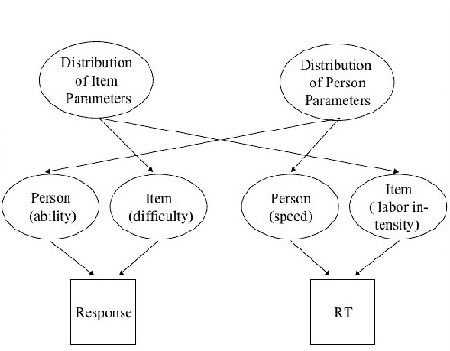
\includegraphics[bb=0 0 450 351]{1.jpg} 
\caption{Двухуровневая иерархическая модель} 
\end{figure}

Как видно, модель имеет два уровня. На первом уровне вероятностные модели для корректности ответа студента и времени ответа студента. На втором уровне вероятностная модель распределения параметров студентов для всех групп обучающихся и вероятностная модель распределения слож\-ностных параметров задачи по всему пулу задач. Рассмотрим эти модели более подробно.

\subsubsection{Двухуровневая иерархическая модель}

\paragraph {Модель распределения параметров для множества студентов (верхний уровень)}

Параметры для группы студентов распределены по нормальному закону
\begin{equation}
(\theta,\tau) \sim N(\mu,\sigma),
\end{equation}
где $\mu = (\mu_\theta, \mu_\tau)^T$ и $\sigma=(\sigma_\theta,\sigma_\tau)$

\paragraph {Модель распределения параметров для множества задач (верхний уровень)}

Введём случайный вектор $\xi$ такой, что $\xi = (a_i,b_i,c_i,\alpha_i, \beta_i)$ - параметры задачи. Тогда
\begin{equation}
\xi \sim N(\mu,\Sigma),
\end{equation}
где $\mu$ - вектор мат. ожиданий и $\Sigma$ - ковариационная матрица для вектора  $\xi$

\paragraph {Модель корректности ответа (нижний уровень)}

Для модели кор\-ректности ответа используется трёхпараметрическая логистическая модель
\begin{equation}
p_i(\theta_j) = c_i - (1-c_i)\psi[a_i(\theta_j - b_i)]б
\end{equation}
где $\psi( * )$ - логистическая функция.

\paragraph {Модель времени ответа (нижний уровень)}
\label{mvonu}

Время ответа студента имеет \\логнормальное распределение:
\begin{equation}
\label{mainmodel}
\ln T_{ij} = \mu + \beta_i + \tau_j + \varepsilon_{ij},\quad \varepsilon_{ij} \sim N(0,\sigma^2).
\end{equation}
Соответственно, плотность распределения имеет следующий вид:
\begin{equation}
f(t_{ij};\tau_j,\alpha_i,\beta_i) = \frac{\alpha_i}{t_{ij}\sqrt{2\pi}}exp\left\{ -\frac{1}{2}[\alpha_i(\ln t_{ij} - \{\beta_i + \tau_j\})]^2 \right\},
\end{equation}
где $\alpha_i = \sigma^{-1}$

В модели используются следующие обозначения:
$$
\begin{array}{lll}
\beta_i &-& \mbox{временной параметр, индивидуальный для задачи i}\\
\tau_j &-& \mbox{параметр времени, в течении которого студент реагирует }  \\
& &\mbox{ на задачи теста }\\
\varepsilon_{ij} &-& \mbox{случайное отклонение}\\
\mu &-& \mbox{параметр времени, общий для всего пула задач и всех обучающихся}
\end{array}
$$

адаптация системы дистанционного обучения с использованием времени \\ответа обучающегося проходит с использованием модели (\ref{mainmodel})

\subsubsection{Оценка параметров модели}
\label{opm}

Пусть в сиcтеме дистанцинного обучения выбирает для формирования вариантов теста используется пул из $N$ задач. При этом в тестировании принимают участие $M$ студентов. Для каждого студента $j$ из общего числа студенов система дистанционного обучения формирует вариант из $n$ задач. Обозначим $t_{ij}$ этом время ответа студента $j$ на задачу $i$. Тогда для случайных параметров модели (\ref{mainmodel}) можно получить оценки методом макси\-мального правдоподобия:
\begin{equation}
\hat{\mu} = \frac{\sum\limits_{j=1}^{M}\sum\limits_{i=1}^{n}\ln t_{ij}}{n \cdot M},
\end{equation}
\begin{equation}
\hat{\beta}_i = \frac{\sum\limits_{j=1}^{M}\ln t_{ij}}{M} - \hat{\mu},
\end{equation}
\begin{equation}
\hat{\tau}_j = \frac{\sum\limits_{i=1}^{n}\ln t_{ij}}{n} - \hat{\mu},
\end{equation}
Оценка $\hat{\tau}_j$ имеет математическое ожидание
\begin{equation}
\label{exp}
E[\hat{\tau}_j] = \tau_j
\end{equation}
и дисперсию
\begin{equation}
\label{var}
Var(\hat{\tau}_j) = \frac{\sigma^2}{n}
\end{equation}
и, наконец, оценка для дисперсии случайного отклонения $\varepsilon_{ij}$ имеет вид
\begin{equation}
\hat{\sigma}^2 = \frac{\sum\limits_{j=1}^{M}\sum\limits_{i=1}^{n}\ln t_{ij} - \hat{\tau}_j - \hat{\beta}_i}{n \cdot M},
\end{equation}

\subsection{Прогнозирование времени ответа пользователя}

Для прогнозирования времени ответа в модели используется подход, опи\-санный ниже.

Обозначим прогнозное время ответа как $\tilde{T}_{ij}$. Тогда с учётом формул \\(\ref{exp}),(\ref{var}) получаем
\begin{equation}
\hat{\tau}_j \sim N\left(\tau_j, \frac{\sigma^2}{n-1}\right)
\end{equation}
т.к.
\begin{equation}
cov(\hat{\tau}_j,\varepsilon_{ij}) = 0,
\end{equation}
то получаем прогнозное время ответа студента на задачу
\begin{equation}
\label{predictedtime}
\ln \tilde{T}_{ij} \sim N\left(\mu + \beta_i + \tau_j,\frac{n\sigma^2}{n-1}\right)
\end{equation}

Таким образом, прогнозное время ответа студента на задачу имеет гаус\-совское распределение.